\documentclass{article}

\usepackage{times}
\usepackage{geometry}
\geometry{a4paper,left=0.6cm,right=0.7cm,top=2cm,bottom=1cm,columnsep=0.8cm}
\usepackage{fontawesome}
\usepackage[hidelinks]{hyperref}
\usepackage{multicol}
\usepackage{tikz}
\usepackage{hyphsubst}
\usepackage{moresize}
\usepackage{hyphenat}
\usepackage{tabularx}
\usepackage{xcolor}
\usepackage{enumitem}

\newcolumntype{Y}{>{\RaggedRight\arraybackslash}X}

\usepackage{enumitem}
\setlist[itemize]{itemsep=1pt,leftmargin=*,topsep=-10pt}

\definecolor{maincolor}{HTML}{f0fafc}
\definecolor{seccolor}{HTML}{ffffff}
\definecolor{gray}{HTML}{8c94a9}
\definecolor{sidetext}{HTML}{59cee5}

\usepackage[contents={}]{background}
\AddEverypageHook{\begin{tikzpicture}[remember picture,overlay]%
  \node[inner sep=0pt,outer sep=0pt] at (current page.north west) [anchor=north west]{%
  \fcolorbox{maincolor}{maincolor}{%
\begin{minipage}[t][\paperheight][t]{0.3\paperwidth}
        \color{white}
        \hspace{0.08cm}
\end{minipage}}
\fcolorbox{seccolor}{seccolor}{
\begin{minipage}[t][\paperheight][t]{0.67\paperwidth}
        \color{black}
        \hspace{1cm}
\end{minipage}
}
  };%
\end{tikzpicture}
}

\usepackage{enumitem}
\setlist[itemize]{itemsep=-2pt,topsep=0pt,leftmargin=1.08cm}
\renewcommand{\labelitemi}{\textcolor{sidetext}{\footnotesize$\bullet$}}

\setlength{\parindent}{0pt}
\usepackage{paracol}

\begin{document}

\pagestyle{empty}

\columnratio{0.3}
\begin{paracol}{2}
\color{sidetext}
\begin{center}
            \begin{tikzpicture}
            \clip (0,0) circle (1.5cm) node[anchor=center] {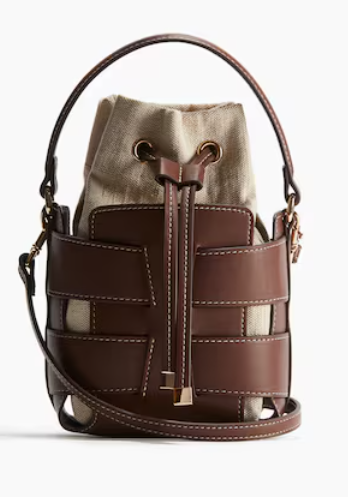
\includegraphics[width=3cm]{da78f51dbd1b4e06a965b418715aaeae.png}}; 
            \end{tikzpicture}

            ~

         {\color{black}\LARGE \textbf{Pape Saliou FALL}}

         ~

         {\large{Data Scientist}}

        
        \end{center}

{\color{gray}\rule{\linewidth}{0.4pt}} \\

 \begin{tabular}{cl}
            \faPhone{}      & 
            \begin{tabular}{p{0.7\linewidth}}
            {\color{gray}Phone}\\
            {0753481453}
            \end{tabular}
            \\ \\
               \faLinkedin{}      & 
            \begin{tabular}{p{0.7\linewidth}}
            {\color{gray}LinkedIn}\\
            {\href{https://www.linkedin.com/in/pape-saliou-fall-43154a211}{https://www.linkedin.com/in/pape-saliou-fall-43154a211} }
            \end{tabular}
            \\ \\
               \faMapMarker{}      & 
            \begin{tabular}{p{0.7\linewidth}}
            {\color{gray}Address}\\
            {Paris, France}
            \end{tabular}
            \\ \\
               \faGlobe{}      & 
            \begin{tabular}{p{0.7\linewidth}}
            {\color{gray}Website/Blog}\\
            {\href{}{ }}
            \end{tabular}
            \\
        \end{tabular}
        \vspace{.2cm} \\
        {\color{gray}\rule{\linewidth}{0.4pt}} \\

        {\color{black}{Languages}}

        ~
        
        \begin{tabular}{cl}
            {\Large\faLanguage{}} & \begin{tabular}{l}
             {Français, Anglais} \\
             {\color{gray}Courant}
            \end{tabular} \\
        \end{tabular}
        \vspace{10pt} \\
        {\color{gray}\rule{\linewidth}{0.4pt}} \\

        \vspace{.4cm}

        {\color{black}{Key Skills}}

        ~
        
        \begin{tabular}{ll}
         \begin{minipage}{0.1\linewidth}
         
\includegraphics[width=\linewidth]{picon.png}
         \end{minipage} & {Python} \\[10pt]
         \begin{minipage}{0.1\linewidth}
         
\includegraphics[width=\linewidth]{picon.png}
         \end{minipage} & {R} \\[10pt]
         \begin{minipage}{0.1\linewidth}
         
\includegraphics[width=\linewidth]{picon.png}
         \end{minipage} & {SQL} \\[10pt]
         \begin{minipage}{0.1\linewidth}
         
\includegraphics[width=\linewidth]{picon.png}
         \end{minipage} & {Machine Learning} \\[10pt]
         \begin{minipage}{0.1\linewidth}
         
\includegraphics[width=\linewidth]{picon.png}
         \end{minipage} & {Deep Learning} \\[10pt]
        \end{tabular}
        
\switchcolumn
\color{black}

\textcolor{black}{\Large \textbf{Professional Summary}} \\

\textcolor{black}{Data Scientist passionn\'e par l’exploitation des donn\'ees pour cr\'eer de la valeur m\'etier. Solide exp\'erience en mod\'elisation statistique, machine learning et visualisation de donn\'ees, acquise lors de projets en finance et t\'el\'ecom. Habitu\'e \`a collaborer avec des \'equipes pluridisciplinaires pour transformer les besoins business en solutions data concrètes et d\'eployables.}\\[8pt]

\textcolor{black}{\Large \textbf{Work Experience}} \\

\colorbox{maincolor}{%
  \begin{minipage}{\linewidth}
    \begin{tabular}{@{}lp{0.72\linewidth}r}
      \begin{minipage}{0.05\linewidth}
        
\includegraphics[width=\linewidth]{picon.png}
      \end{minipage} & 
      {Prepaya} &  
      {\footnotesize {Jan 2022} {-- Dec 2023} } \\[-10pt]
      & {\color{sidetext}{Data Scientist}} & \\
      & {\small {Paris, France}} & \\
    \end{tabular}
\begin{itemize}
    \item D\'evelopp\'e des mod\`eles de pr\'ediction de churn am\'eliorant la r\'etention de 15\,\%, automatis\'e des pipelines ETL avec Python et Airflow r\'eduisant le temps de traitement de 40\,\%, con\c{c}u des dashboards Power~BI pour le suivi des KPI, et collabor\'e avec les \'equipes produit et marketing pour transformer les insights data en actions concr\`etes.
\end{itemize}
  \end{minipage}%
}

~ \\[-6pt]

\colorbox{maincolor}{%
  \begin{minipage}{\linewidth}
    \begin{tabular}{@{}lp{0.72\linewidth}r}
      \begin{minipage}{0.05\linewidth}
        
\includegraphics[width=\linewidth]{picon.png}
      \end{minipage} & 
      {} &  
      {\footnotesize {} {} } \\[-10pt]
      & {\color{sidetext}{}} & \\
      & {\small {} } & \\
    \end{tabular}
\begin{itemize}
    \item 
\end{itemize}
  \end{minipage}%
}


\vspace{1cm}

\textcolor{black}{\Large \textbf{Education}} \\


 \begin{tabular}{@{}cp{0.7\linewidth}}
      \begin{minipage}{0.05\linewidth}
        
\includegraphics[width=\linewidth]{picon.png}
      \end{minipage} & \vspace{-12pt}
      {\color{sidetext} {Master 2 Data science}} \\[-6pt]
      & {k dqvkbbqsv  vqdvklbq} \\
      & {Data Science} \\
      & {2022-2023} 
    \end{tabular}


~

~

 \begin{tabular}{@{}cp{0.7\linewidth}}
      \begin{minipage}{0.05\linewidth}
        
\includegraphics[width=\linewidth]{picon.png}
      \end{minipage} & \vspace{-12pt}
      {\color{sidetext} {}} \\[-6pt]
      & {} \\
      & {} \\
      & {} 
    \end{tabular}

\vspace{0.5cm}

\textcolor{black}{\Large \textbf{Certifications}} \\

\begin{itemize}[leftmargin=12pt]
\item Jul-2024 -- ksLD  (KSLQKBC)
\item 
\end{itemize}


\end{paracol}



\end{document}